\begin{frame}[allowframebreaks]{Transformers}
    \begin{figure}
        \centering
        \includegraphics[width=\linewidth,height=\textheight,keepaspectratio]{images/transformers/slide_55_1_img.png}
    \end{figure}

    \framebreak

    \begin{columns}
        \begin{column}{0.55\textwidth}
            \begin{figure}
                \flushleft
                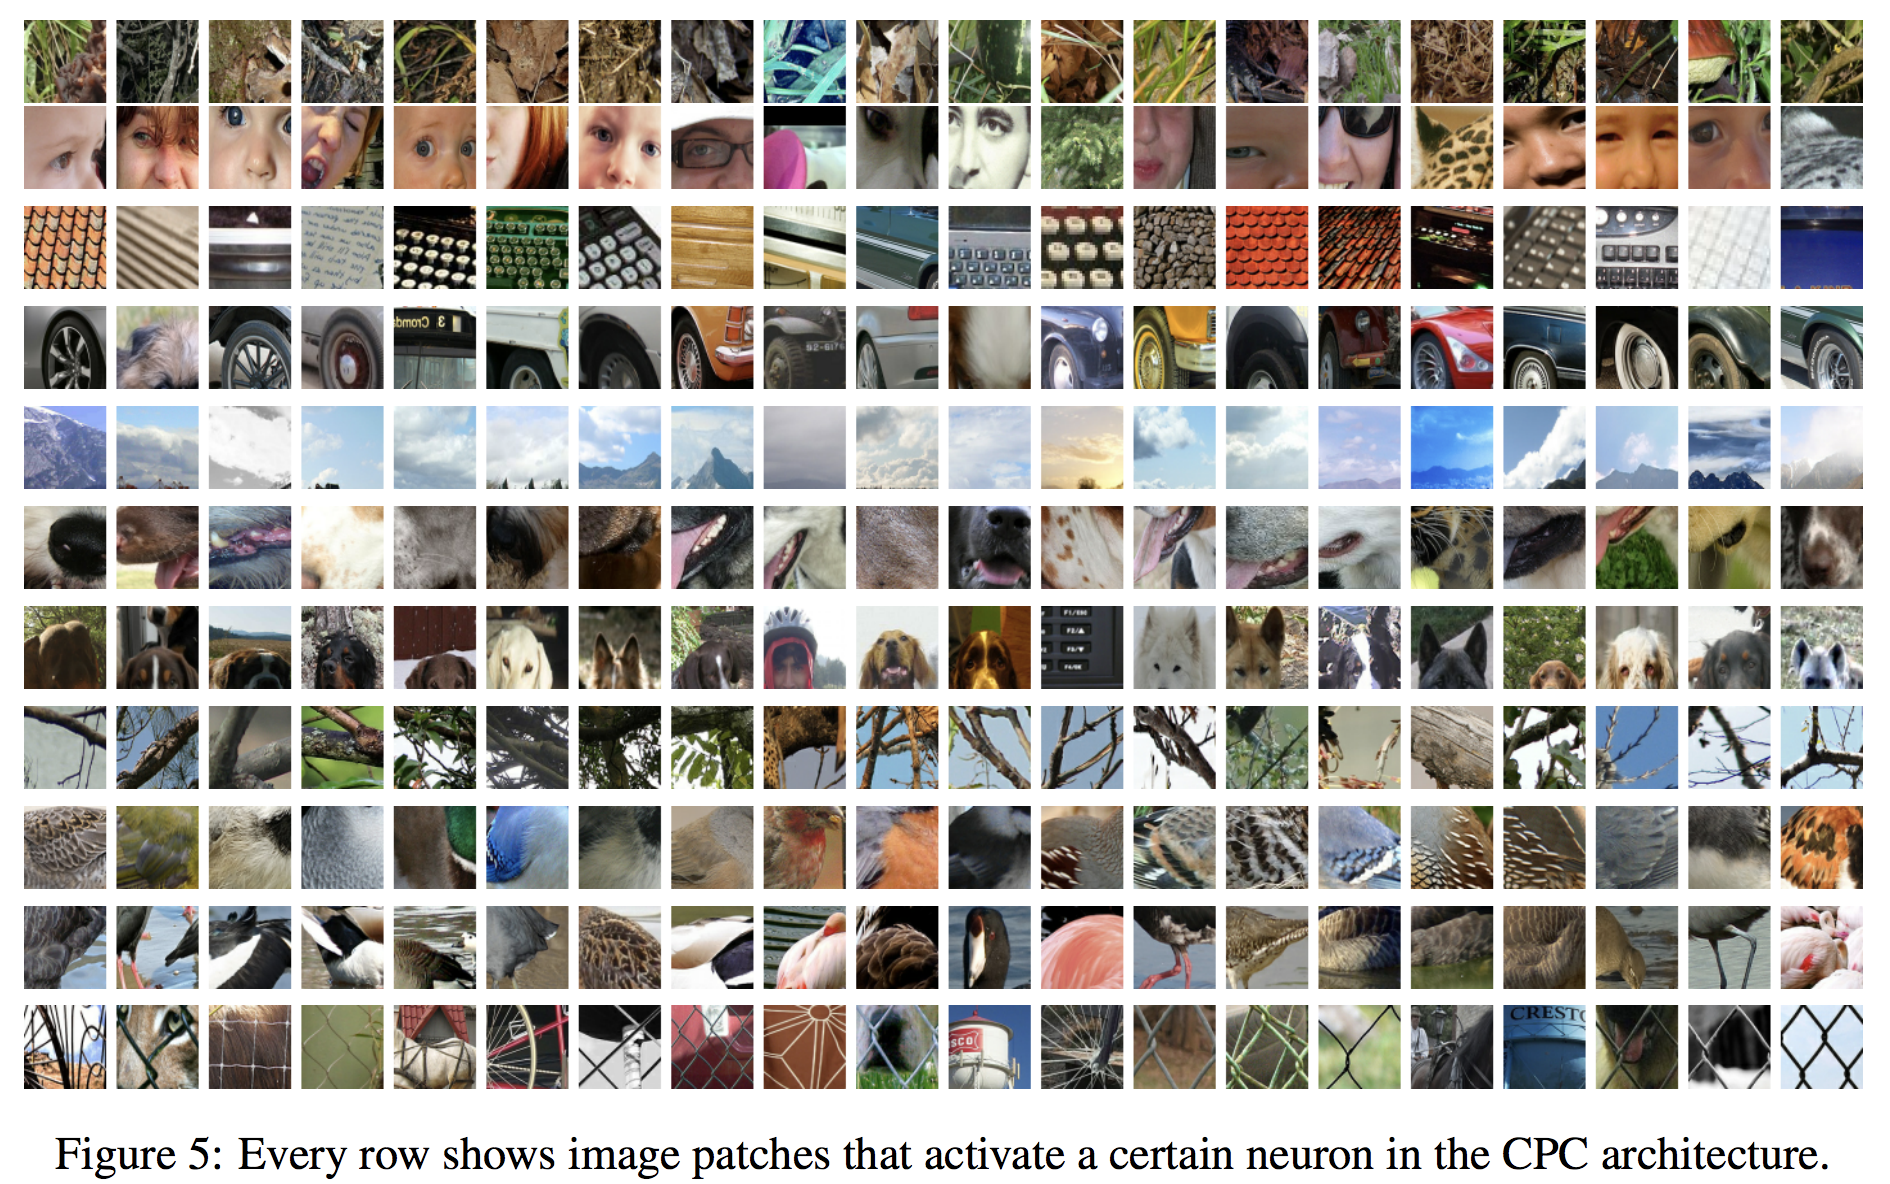
\includegraphics[width=\linewidth,height=\textheight,keepaspectratio]{images/transformers/slide_56_1_img.png}
                \caption{Detailed view of a single Transformer block.}
            \end{figure}
        \end{column}
        \begin{column}{0.45\textwidth}
            \begin{itemize}
                \item \textbf{Input:} A set of vectors $\mathbf{x}$, one per token.
                \item \textbf{Output:} A set of vectors $\mathbf{y}$, one per token.
                \item \textbf{Self-Attention:} Allows each token to attend to all others, capturing contextual relationships.
                \item \textbf{Layer Normalization \& MLP:} Applied independently to each token, ensuring stability and expressiveness.
                \item \textbf{Key Properties:} Highly scalable and parallelizable due to independent operations across tokens.
            \end{itemize}
        \end{column}
    \end{columns}

    \framebreak

    \begin{figure}
        \flushleft
        \includegraphics[width=\linewidth,height=\textheight,keepaspectratio]{images/transformers/slide_57_1_img.png}
        \caption{Stacking multiple Transformer blocks.}
    \end{figure}
    \vspace{-0.2em}
    \begin{itemize}
        \item A Transformer consists of a sequence of identical blocks, each refining the token representations.
        \item In the original architecture (Vaswani et al., 2017): 12 blocks, hidden size $D_Q = 512$, and 6 attention heads were used.
        \item The modular design enables deep stacking and efficient parallel computation.
    \end{itemize}
\end{frame}